The SCE regards a natural  evolution happening
simultaneously in independent communities.
The algorithm works with a population partitioned in $N$ complexes, each one
having $M$ individuals.
Initially the population of $N*M$ individuals is randomly taken from the
feasible solution space.
After this initialization the population is sorted by descending order according
to their fitness and the best global solution is identified.
The entire population is then partitioned (shuffled) into $N$ complexes,
each containing $M$ individuals.
In this shuffling process the first individual goes to the first complex, the second
individual goes to the second complex, individual $N$ goes to $N$-th complex,
individual $(M+1)$-th goes back to the first complex, etc.

The next step after shuffling the complexes is to evolve each complex through
a given fixed amount of $K'$ steps.
The individuals in each complex are sorted by descending order of fitness.
In each step a subcomplex of $P$ individuals is selected from the
complex using a triangular probability distribution, where the $i$-th individual
has a probability $p_i = \frac{2(n+1-i)}{n(n+1)}$ of being selected.
The use of triangular distribution is intended to prioritize individuals with
better fitness, supporting the algorithm convergence rate.

After the selection of the subcomplex, its worst individual is identified to
be replaced by a new generated solution.
This new solution is generated by the crossing of the worst individual and an
other individual with better fitness.
At first the best individual of the subcomplex is considered for the crossing.
If the new solution is not better than the worst one, the best individual
of the complex is considered for a crossing.
If the latter crossing did not result in any improvement, the best individual
of whole population is considered.
Finally, if all the crossing steps couldn't generate a better individual,
the worst individual of the subcomplex is replaced by a new random solution taken
from the feasible solution space.
This last step is important to prevent the algorithm becoming trapped in local minima.
Figure~\ref{fig:flow2} presents the evolving procedure described above in a flowchart diagram.

After evolving all the $N$ complexes the whole population is again
sorted by descending order of fitness and the process continues until
a stop condition is satisfied.
Figure~\ref{fig:flow1} shows the SCE algorithm in a flowchart diagram in which
the stop condition is a fixed amount of $K$ evolving steps.

\begin{figure}
\begin{algorithmic}[1]
  \Procedure{New random solution}{}
    \State $v \leftarrow $ shuffle($1, 2, \ldots, n$)
	\State $s \leftarrow \emptyset$ \Comment{empty solution}
    \For{$ i \leftarrow 1:n$ }
	  \State $s \leftarrow s \cup \{v_i\}$ \Comment{adding item}
	  \If{ $s$ is not feasible} \Comment{checking feasibility}
	    \State $s \leftarrow s - \{v_i\}$
      \EndIf
	\EndFor
  \State return $s$
  \EndProcedure
\end{algorithmic}
\caption{Generation of a new random solution for the MKP.}
\label{alg:new}
\end{figure}


\begin{figure}[!tbp]
  \centering
  \begin{minipage}[b]{0.4\textwidth}
    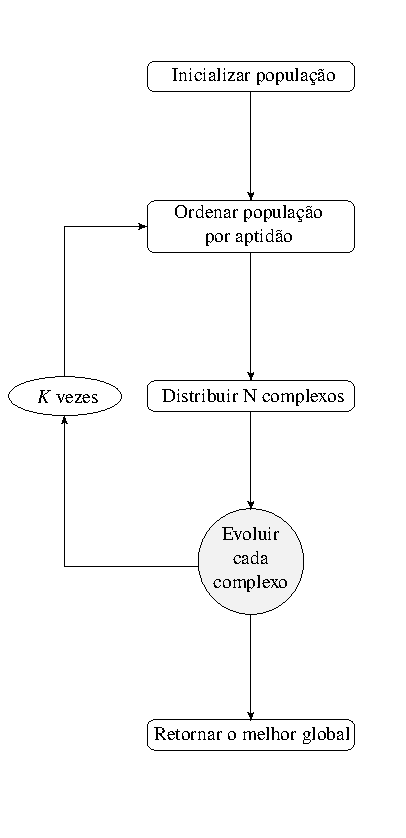
\includegraphics[width=\textwidth]{img/sce/flow1}
    \caption{The shuffled complex evolution algorithm.}
    \label{fig:flow1}
  \end{minipage}
  \hfill
  \begin{minipage}[b]{0.4\textwidth}
    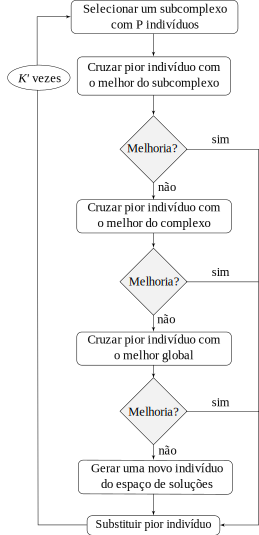
\includegraphics[width=\textwidth]{img/sce/flow2}
    \caption{The evolving stage of SCE for a single complex.}
    \label{fig:flow2}
  \end{minipage}
\end{figure}
